\documentclass[10pt,a4paper]{article}
\usepackage{setspace}
\usepackage{parskip}
\usepackage{amsmath, amssymb}
\usepackage{titlesec}
\usepackage[utf8]{inputenc}
\usepackage{enumitem}
\usepackage{tocbibind} % Para incluir o sumário no índice
\usepackage[T1]{fontenc}
\usepackage{xcolor}
\usepackage{tcolorbox}
\usepackage{enumitem}
\usepackage{algorithm}
\usepackage{algpseudocode}
\usepackage{amsmath}
\usepackage{fancybox}
\usepackage{color}
\usepackage{framed}
\usepackage{ragged2e}
\usepackage{fancyhdr}
\usepackage{amsmath}
\usepackage[justification=centering]{caption}
\usepackage{tabularx}  % Para tabelas com largura variável
\usepackage{hyperref}
\usepackage{array} % Para usar o comando \newcolumntype
\usepackage{siunitx}
\usepackage{enumitem}
\usepackage{fancyhdr}
\usepackage{lipsum} % Pacote para geração de texto de exemplo
\usepackage{lipsum} % Pacote para gerar texto de exemplo
\usepackage{caption}
\usepackage{array}  % Para ajustar a largura das colunas
\usepackage{booktabs}  % Para linhas horizontais mais bonitas
\usepackage{caption}  % Para legenda da tabela
\usepackage{cite}
\captionsetup{justification=justified, singlelinecheck=false}
\usepackage{subcaption} % Pacote para criar subfiguras
\usepackage{float}% Package for precise float placement
\usepackage[table]{xcolor} % Required for \cellcolor
\usepackage{colortbl}      % Additional table color support
\usepackage{booktabs}      % For better table lines
\usepackage{float}         % For [H] positioning
\usepackage[draft]{graphicx}
\usepackage{caption}
\usepackage{pdfpages}
 


\usepackage[top=2cm, bottom=2cm, left=3cm, right=3cm]{geometry}
\usepackage{setspace}
\usepackage{parskip}
\usepackage{titlesec}
\usepackage{enumitem}
\usepackage{hyperref} % Para links de email

% Configurações de espaçamento e títulos
% Espaçamento antes e depois
\titlespacing{\section}{0pt}{*2}{*2}
\titlespacing{\subsection}{0pt}{*1.5}{*1.5}
\titlespacing{\subsubsection}{0pt}{*1}{*1}
\setlength{\parskip}{4pt}
\setlength{\abovedisplayskip}{0pt}
\setlength{\belowdisplayskip}{0pt}
\setstretch{1}




% Configuração de lista com espaço entre itens
\setlist[enumerate]{itemsep=1pt} % Espaço de 6pt entre itens de enumerate

% Pacote para verificar se a página é par ou ímpar
\usepackage{changepage}
\usepackage[justification=centering]{caption}

\begin{document}

% Capa
\begin{titlepage}
    \centering
    \vspace*{\fill} % Início da centralização vertical
    {\LARGE\bfseries Predicting Stock Price Movements utilizing LSTM Networks\par}
    \vspace{1cm} % Espaço entre o título e o subtítulo
    % Subtítulo em itálico
    \vspace{2cm}
    {\Large\bfseries Guilherme Grancho Duarte Fernandes\par}
    \vspace{0.5cm} % Espaço entre o nome e a afiliação
    {\large Department of Physics, Instituto Superior Técnico, Lisbon, Portugal\par}
    {\large \href{mailto:guilhermegrancho@tecnico.ulisboa.pt}{guilhermegrancho@tecnico.ulisboa.pt}\par}
    \vspace{1cm} % Espaço entre os autores
    {\Large\bfseries Vasco Vieira Rosado Serpa Pereira\par}
    \vspace{0.5cm}
    {\large Department of Computer Science and Engineering, Instituto Superior Técnico, Lisbon, Portugal\par}
    {\large \href{mailto:talles@ufop.edu.br}{vasco.serpa.pereira@tecnico.ulisboa.pt}\par}
    \vspace{3cm} % Espaço entre os autores e a data
    {\large March 2025\par}
    \vspace*{\fill} % Final da centralização vertical
\end{titlepage}

% Definindo novas cores
\definecolor{lightgray}{gray}{0.9}
\definecolor{darkgray}{gray}{0.3}

% Página para o Abstract
\newpage

% Abstract
\section*{Abstract}
\addcontentsline{toc}{section}{Abstract}

\noindent\rule{\textwidth}{1pt}
\vspace{0.1mm}

This paper showcases the effectiveness of Long Short-Term Memory (LSTM) networks in predicting stock price movements with high accuracy, emphasizing the critical role of selecting appropriate training metrics for optimizing such models. We analyze the performance of five stocks and three exchange-traded funds (ETFs) retrieved through the Alpaca API. The data spans from January 1, 2016, to December 30, 2024, offering a diverse perspective that captures a wide range of market conditions, trends, and volatility patterns.
Our approach is based on the use of two metrics as input to the model: the Volume Weighted Average Price (VWAP) and the Trade Count. The predictions are generated at three-hour intervals, which facilitates a detailed examination of short-term trends.
In general, this study not only demonstrates the robustness of LSTM networks in financial forecasting, but also offers valuable insights to researchers and investors alike looking to improve their decision making in the stock market.

\vspace{0.5mm}
\noindent\rule{\textwidth}{1pt}

\textbf{KeyWords:} Long Short-Term Memory (LSTM), Stock Market, Recurrent Neural Network 

\newpage


%Introdução
\section{Introduction}

Investing successfully in the stock market has long been an unpredictable and challenging endeavor. According to the Efficient Market Hypothesis (EMH), asset prices fully reflect all available information, suggesting that consistently outperforming the market is nearly impossible if it is truly efficient. However, the rise of machine learning—particularly deep neural networks like Recurrent Neural Networks (RNNs) and their advanced variant, Long Short-Term Memory (LSTM)—offers new possibilities for analyzing and predicting market behavior by detecting nonlinear patterns in time series that traditional models often miss.

In this paper, we employ an LSTM-based approach to model and forecast short-term stock price movements. Unlike conventional feedforward networks, LSTMs excel at retaining temporal dependencies across time steps, making them ideal for sequential financial data. To enrich our model’s inputs, we incorporate two technical indicators: Volume Weighted Average Price (VWAP) and Trade Count. These metrics capture real-time trading behavior and market microstructure dynamics, potentially revealing subtle patterns hidden in raw price data.

Our goal is to empirically evaluate whether this LSTM model can challenge the EMH by demonstrating predictive power across diverse financial instruments. We hypothesize that LSTMs, using VWAP and Trade Count, can detect short-term price inefficiencies, particularly in volatile markets, thus questioning the universality of the EMH. The study spans five major technology stocks and three prominent exchange-traded funds (ETFs) from January 1, 2016 to December 30, 2024, a period that includes bull markets, corrections, and increased volatility.

To test this model rigorously, we compare two data sources: the SIP feed, which includes full-day trading (pre-market and post-market hours), and the IEX feed, limited to regular trading hours. Extended-hours data from the SIP feed may capture early market reactions to news, potentially improving predictions compared to regular-hours IEX data. By training separate models on each feed, we assess the value of including extended-hours activity.

We also explore the impact of data normalization on model performance. Given financial data’s outliers and non-stationary nature, we test three scalers: Standard Scaler, MinMax Scaler, and Robust Scaler to identify the best approach for stabilizing inputs and enhancing model accuracy.

Finally, predictions are made at three-hour intervals to capture intraday market dynamics. This interval aligns with short-term trading cycles, allowing actionable forecasts while reflecting intraday volatility. This granularity is especially relevant for short-term traders and high-frequency strategies, where timely and accurate predictions are critical.


%Papers Relacionados
\section{Related Works}

This section discusses related work, particularly highlighting studies that utilize LSTM networks and VWAP as an indicator.

Moghar and Hamiche (2020) \cite{moghar2020stock} conducted a study employing LSTM models to predict stock market values, emphasizing the capability of machine learning techniques to model non-linear patterns effectively. They highlighted that LSTM significantly outperformed traditional linear models like ARIMA in predictive accuracy, especially with financial time series data characterized by high volatility and non-linearity. Their analysis underlined how LSTM models could enhance precision by learning temporal dependencies that traditional forecasting methods might overlook.

Further expanding on the capabilities of LSTM networks, Shen and Shafiq (2020) \cite{shen2020shortterm} proposed a comprehensive deep learning-based system tailored specifically for short-term stock market price trend prediction. Their approach incorporated extensive feature engineering and customization of the LSTM architecture. By conducting experiments with two years of data from the Chinese stock market, they demonstrated significant improvement in predictive accuracy due to their detailed feature engineering process, which proved crucial in refining model performance. Their results suggested that carefully engineered features could notably augment the predictive power of deep learning models.

Regarding the application of the VWAP, Zarattini and Aziz (2023) \cite{zarattini2023vwap} explored its efficacy as a day trading indicator for detecting market imbalances and making trading decisions. Using VWAP, they developed a straightforward day trading strategy that initiated long positions when the price was above VWAP and short positions when below it. Their study, involving trading instruments like QQQ and TQQQ over several volatile market periods from 2018 to 2023, showed substantial profitability and superior risk-adjusted returns compared to traditional buy-and-hold strategies. Notably, the VWAP-based strategy significantly reduced the maximum drawdown and provided robust returns across diverse market conditions.

Collectively, these studies emphasize the potential of combining advanced LSTM and hybrid architectures with strategically selected trading indicators such as VWAP. The literature clearly indicates that deep learning models, particularly LSTM, are highly effective for capturing complex patterns within financial data, while the VWAP indicator provides significant insights into real-time market trading behaviors. These findings form a critical foundation for the current research, which integrates these concepts to explore new dimensions of stock market predictability and market efficiency debates.



%Métodos e Materiais
\section{Methods and Materials}

%Data
\subsection{Data}

To explore diverse market dynamics and ensure a comprehensive evaluation, we chose to build individual LSTM models for each of the following companies and indexes: Nvidia (NVDA), Apple (AAPL), Microsoft (MSFT), Amazon (AMZN), Alphabet (GOOG), the S\&P500 (VOO), the Dow Jones Industrial Average (DIA) and the Russel 2000 (IWM). These selections were made because they represent the five largest companies in the world by market capitalization and three of the most significant stock market indices, providing a well-rounded perspective on both individual stock performance and broader market trends. 

All data is retrieved through the Alpaca Trading API \cite{alpaca_api}, using the SIP (Securities Information Processor) data source, covering the period from January 1, 2016, to December 30, 2024 and contains information not only about regular trading hours but also pre-market and after-hours trading.  Although we will only utilize the VWAP and trade count, the Alpaca API also provides open, close, high, low, and volume information for each interval. The data is retrieved at 5-minute intervals to capture fine-grained intraday price movements and trading behaviors effectively.

To ensure an effective training process and robust model evaluation, the data is divided into three subsets: 60\% is allocated for training, 20\% for validation, and the remaining 20\% is reserved for testing. This division allows the model to learn effectively, tune hyperparameters without overfitting, and assess its predictive performance accurately on unseen data.

\subsection{Features}

\subsubsection{Volume Weighted Average Price}

The Volume Weighted Average Price (VWAP) is a trading benchmark that reflects the average price a security has traded at throughout a specific period, weighted by the volume of each trade. It is widely used by institutional traders to assess market trends and trading performance. VWAP is particularly useful because it integrates both price and volume information, offering a more accurate representation of where most of the market activity occurred.

VWAP for a given time period is calculated using the formula:
\begin{equation}
\text{VWAP} = \frac{\sum_{i=1}^{n} P_i \cdot V_i}{\sum_{i=1}^{n} V_i}
\end{equation}
where $P_i$ is the price of the $i$-th trade (or average of high, low, and close), and $V_i$ is the corresponding trade volume. The summation runs over all trades in the given interval. In our study, VWAP is computed at 5-minute intervals and serves as a core input feature to the LSTM model, helping identify periods of high market consensus, potential support/resistance zones, and intraday price dynamics.

\subsubsection{Trade Count}

Trade Count represents the total number of executed trades within a 5-minute interval. Unlike volume, which reflects the number of shares traded, trade count focuses on the frequency of transactions. This metric helps capture market activity in a different dimension — highlighting periods of high-frequency trading or increased market participation. When used alongside VWAP, trade count contributes to understanding the behavioral dynamics of the market, potentially indicating breakout zones or consolidation periods. In our model, it acts as a complementary input feature to enhance short-term price movement predictions.

\subsection{Data Sources and Market Hours}

To evaluate the effect of extended trading hours on prediction performance, we trained and compared models using two distinct data sources:

\begin{itemize}
    \item \textbf{SIP (Securities Information Processor)}: Provides full-day trading data, including pre-market (before 9:30 AM) and post-market (after 4:00 PM) sessions. This feed captures institutional and retail activity occurring outside standard trading hours.
    
    \item \textbf{IEX (Investors Exchange)}: Offers data restricted to regular trading hours (9:30 AM to 4:00 PM), excluding off-hours activity. This feed reflects more stable and regulated trading conditions.
\end{itemize}

Each model was trained separately using identical architecture and scaling techniques to isolate the effect of the data source. Comparative performance was evaluated based on accuracy, loss and confusion matrix metrics.


\subsection{Scalers}

In this study, we investigated the impact of different feature scaling techniques on the predictive performance of our models. Specifically, we utilized three distinct scaling methods — Standard Scaler, MinMax Scaler, and Robust Scaler — all implemented using the scikit-learn Python library \cite{scikit-learn}. 
The Standard Scaler standardizes features by removing the mean and scaling to unit variance, thus normalizing data with an assumption of Gaussian distribution. The MinMax Scaler transforms features by scaling each feature to a specified range, typically [0,1], which helps handle features with significant differences in magnitudes. The Robust Scaler, on the other hand, scales features based on the median and interquartile range, making it particularly effective in handling outliers.

We applied each scaler individually to the VWAP values of each stock, systematically comparing their predictive performance against a baseline model without any scaling. This comprehensive evaluation enabled us to identify the most effective scaling technique, improving model accuracy and robustness across varying market conditions and stock behaviors.

\subsection{Neural Networks}

\subsubsection{Recurrent Neural Networks}

Recurrent Neural Networks (RNNs) are a specialized class of neural networks designed to process sequential data. Unlike traditional feedforward neural networks, RNNs feature recurrent connections that create cycles, enabling them to maintain a ``memory'' of previous inputs. This characteristic makes them well-suited for tasks where the order of data points is significant, such as time series analysis, natural language processing, and financial forecasting.

In an RNN, the network processes each element of a sequence using a shared set of weights. At each time step \( t \), the hidden state \( h_t \) is updated based on the current input \( x_t \) and the previous hidden state \( h_{t-1} \), as described by the equation:

\[ h_t = \sigma(W_h h_{t-1} + W_x x_t + b) \]

where \( \sigma \) is an activation function (for example, tanh or sigmoid), \( W_h \) and \( W_x \) are weight matrices for the hidden state and input, respectively, and \( b \) is a bias term. The output \( y_t \) is then computed as:

\[ y_t = W_y h_t + b_y \]

where \( W_y \) and \( b_y \) are the weight matrix and bias for the output layer. This architecture allows RNNs to theoretically capture temporal dependencies by passing information forward through the sequence.

RNNs are trained using Backpropagation Through Time (BPTT), which extends traditional backpropagation to account for the sequential nature of the data. However, while RNNs excel at handling short-term dependencies, they often struggle with long-term dependencies due to the exploding and vanishing gradients problem, which limits their effectiveness in applications requiring extended memory.

\subsubsection{The Exploding and Vanishing Gradients Problem}

The exploding and vanishing gradients problem poses a significant obstacle when training RNNs, especially for long sequences. During BPTT, gradients are computed by unrolling the network across time steps and propagating errors backward. This process can lead to two issues:

\begin{itemize}
    \item \textbf{Exploding Gradients}: When gradients grow exponentially large, they cause drastic weight updates, destabilizing training. This can be addressed through techniques like gradient clipping, which caps gradient values above a threshold.
    \item \textbf{Vanishing Gradients}: When gradients shrink exponentially, they become too small to influence weight updates effectively, preventing the network from learning long-term dependencies. This occurs because repeated multiplications of small weight values diminish the gradient as it propagates backward.
\end{itemize}

In financial time series prediction, where long-term trends can be critical, the vanishing gradients problem severely hampers RNN performance. To overcome this limitation, advanced architectures such as LSTM networks have been developed.

\subsubsection{Long Short-Term Memory}

Long Short-Term Memory (LSTM) networks are a specialized type of RNN designed to mitigate the vanishing gradients problem and effectively capture long-term dependencies in sequential data. Introduced by Hochreiter and Schmidhuber in 1997 \cite{hochreiter1997}, LSTMs incorporate a memory cell and three key gating mechanisms: input gate, forget gate, and output gate that regulate the flow of information through the network.

The structure of an LSTM unit includes:

\begin{itemize}
    \item \textbf{Memory Cell (\( c_t \))}: Stores information over time, enabling the network to retain critical features across long sequences.
    \item \textbf{Input Gate (\( i_t \))}: Controls how much new information from the current input is added to the memory cell.
    \item \textbf{Forget Gate (\( f_t \))}: Determines how much of the previous memory cell content is discarded.
    \item \textbf{Output Gate (\( o_t \))}: Regulates how much of the memory cell’s content contributes to the output.
\end{itemize}

%These gates use sigmoid activation functions (outputting values between 0 and 1) to filter information selectively. 

%COLOCAR IMAGEM?

These mechanisms allow LSTMs to selectively remember or forget information, making them highly effective for modeling temporal relationships in financial data.

\begin{figure}[h]
\centering
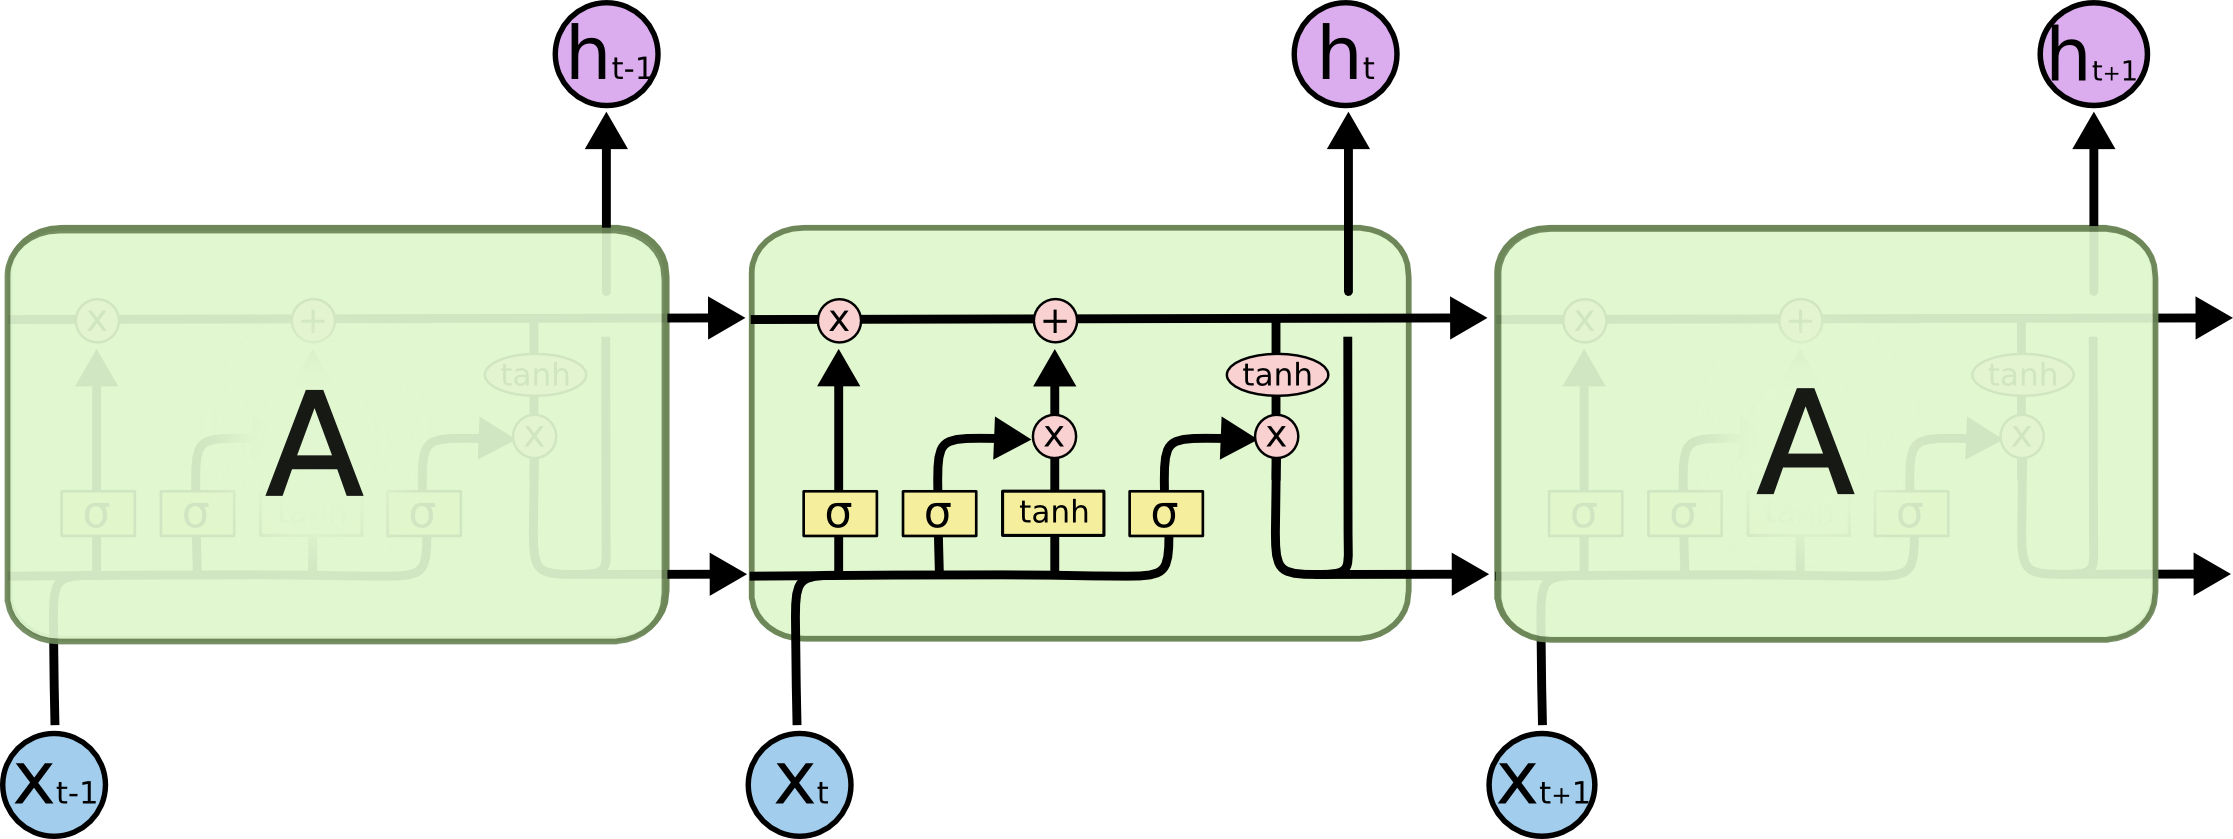
\includegraphics[width=0.8\textwidth]{LSTM-chain.png}
\caption{Internal structure of an LSTM unit, illustrating the flow of data and the gating mechanisms. Inputs  are processed alongside hidden states  and cell states , showcasing how information is selectively retained or discarded. Adapted from \cite{olah2015lstm}.}
\label{fig:lstm_structure}
\end{figure}

In this study, LSTMs are employed to forecast intraday stock price movements based on historical VWAP and trade count data. The model’s ability to capture complex, non-linear dependencies over a 3-hour look-back window makes it an ideal choice for this task. The architecture of the LSTM model is structured as follows:


\begin{itemize}
    \item \textbf{First LSTM Layer}: Contains 64 units and returns the full sequence of outputs, enabling further temporal processing.
    \item \textbf{Dropout Layer}: Applied with a 20\% dropout rate to the first LSTM layer’s output, reducing the risk of overfitting.
    \item \textbf{Second LSTM Layer}: Also with 64 units, this layer processes the sequence from the first layer and outputs only the final hidden state, summarizing the input sequence.
    \item \textbf{Second Dropout Layer}: Another 20\% dropout layer to further regularize the model.
    \item \textbf{Dense Output Layer}: A single-unit layer with a sigmoid activation function, producing the probability that the stock price will increase within the next three hours.
\end{itemize}

The model comprises 50,241 trainable parameters and is trained using BPTT with the Adam optimizer and binary cross-entropy loss function. To prevent overfitting and ensure efficient training, an EarlyStopping callback is employed to monitor validation accuracy, stopping the training process once improvements plateau. The input to the model is a matrix with 36 rows and 2 columns, where each row represents a 5-minute interval containing VWAP and trade count values, spanning a 3-hour look-back window (36 \(\times\) 5 minutes = 180 minutes). The model’s output is a binary label— either 0 or 1 —indicating the predicted directional movement of the stock price in the next time interval, where 0 represents a decrease and 1 an increase. This binary classification approach simplifies the prediction task by focusing solely on the direction of the price movement, rather than attempting to forecast the exact price. % Ultima frase deixo ou nao?

This LSTM architecture leverages its gating mechanisms to retain relevant patterns in the data while discarding noise, enabling accurate predictions of stock price movements. By processing sequences of intraday market data, the model captures the intricate temporal dynamics that drive financial markets, offering a powerful tool for forecasting.


\section{Results}

The performance of the LSTM models was evaluated based on two key metrics: test accuracy and test loss. These metrics were computed for each combination of scaler and ticker. Results are presented separately for the IEX and SIP datasets to investigate the influence of regular trading hours versus extended trading hours on model performance.

\subsection{IEX}

For the IEX dataset, which includes only regular trading hours, the test accuracy and test loss are summarized in Tables 1 and 2, respectively.

\begin{table}[H]
\centering
\definecolor{lightgreen}{RGB}{198, 255, 221}
    \caption{IEX Feed: Test Accuracy by Scaler and Ticker (Including Mean)}
\begin{tabular}{lcccc}
\toprule
\textbf{Ticker} & \textbf{Standard} & \textbf{MinMax} & \textbf{Robust} & \textbf{NoScaler} \\
\midrule
AAPL  & 0.7330 & \cellcolor{lightgreen}{0.7470} & 0.7130 & 0.7300 \\
AMZN  & 0.7430 & 0.7500 & \cellcolor{lightgreen}{0.7540} & 0.6640 \\
DIA   & 0.5420 & 0.6150 & 0.5210 & \cellcolor{lightgreen}{0.6200} \\
GOOG  & 0.6920 & \cellcolor{lightgreen}{0.7070} & 0.6790 & 0.6450 \\
IWM   & 0.6840 & 0.6960 & 0.7010 & \cellcolor{lightgreen}{0.7150} \\
MSFT  & 0.7210 & 0.7350 & \cellcolor{lightgreen}{0.7370} & 0.7190 \\
NVDA  & 0.7450 & \cellcolor{lightgreen}{0.7520} & 0.7350 & 0.7070 \\
VOO   & \cellcolor{lightgreen}{0.6100} & 0.5830 & 0.5980 & 0.5950 \\
\midrule
\textbf{Mean} & 0.6838 & \cellcolor{lightgreen}{0.6981} & 0.6797 & 0.6744 \\
\bottomrule
\label{tab:iex_accuracy}
\end{tabular}
\end{table}

\begin{table}[H]
\centering
\definecolor{lightblue}{RGB}{198, 221, 255}
\caption{IEX Feed: Test Loss by Scaler and Ticker (Including Mean)}
\begin{tabular}{lcccc}
\toprule
\textbf{Ticker} & \textbf{Standard} & \textbf{MinMax} & \textbf{Robust} & \textbf{NoScaler} \\
\midrule
AAPL  & 0.5510 & \cellcolor{lightblue}{0.5430} & 0.5530 & 0.5520 \\
AMZN  & \cellcolor{lightblue}0.5540 & 0.5560 & 0.5840 & 0.8200 \\
DIA   & 0.7270 & 0.6850 & 0.7080 & \cellcolor{lightblue}{0.6590} \\
GOOG  & 0.6560 & \cellcolor{lightblue}{0.5900} & 0.6320 & 0.6850 \\
IWM   & 0.6120 & 0.5980 & 0.6110 &\cellcolor{lightblue} 0.5870 \\
MSFT  & 0.6140 & \cellcolor{lightblue}{0.5360} & 0.5850 & 0.5410 \\
NVDA  & \cellcolor{lightblue}0.5450 & 0.5460 & 0.5490 & 0.6090 \\
VOO   & \cellcolor{lightblue}{0.6730} & 0.6940 & 0.6840 & 0.6800 \\
\midrule
\textbf{Mean} & 0.6165 & \cellcolor{lightblue}{0.5935} & 0.6133 & 0.6416 \\
\bottomrule
\label{tab:iex_loss}
\end{tabular}
\end{table}

\subsubsection*{Key Observations for IEX}

\textbf{Test Accuracy:} The MinMax scaler achieved the highest mean accuracy (0.6981), outperforming Standard (0.6838), Robust (0.6797), and NoScaler (0.6744). At the ticker-specific level, MinMax was optimal for AAPL, GOOG, and NVDA, while the Robust scaler excelled for AMZN and MSFT. NoScaler provided the best accuracy for DIA and IWM, and the Standard scaler was the most effective only for VOO.This variation highlights the importance of selecting appropriate scaling methods based on individual stocks or ETFs.

\textbf{Test Loss:} MinMax also had the lowest mean loss (0.5935), clearly outperforming Standard (0.6165), Robust (0.6133), and NoScaler (0.6416). Ticker-specific analysis shows MinMax performed best for AAPL, GOOG, and MSFT, while NoScaler was optimal for DIA and IWM. Standard scaling achieved the lowest loss values for AMZN, NVDA, and VOO. These results confirm MinMax as generally effective in reducing loss during regular trading hours, despite some exceptions across tickers.



\subsection{SIP}

For the SIP dataset, which includes extended trading hours (pre-market, regular and post-market sessions), the test accuracy and test loss are summarized in Tables 3 and 4, respectively.


\begin{table}[H]
\centering
\definecolor{lightgreen}{RGB}{198, 255, 221}
\caption{SIP Feed: Test Accuracy by Scaler and Ticker (Including Mean)}
\begin{tabular}{lcccc}
\toprule
\textbf{Ticker} & \textbf{Standard} & \textbf{MinMax} & \textbf{Robust} & \textbf{NoScaler} \\
\midrule
AAPL  & 0.8120 & \cellcolor{lightgreen}{0.8250} & 0.8210 & 0.8190 \\
AMZN  & 0.7920 & 0.7920 & \cellcolor{lightgreen}{0.8070} & 0.6660 \\
DIA   & 0.8360 & 0.8400 & \cellcolor{lightgreen}{0.8420} & \cellcolor{lightgreen}{0.8420} \\
GOOG  & \cellcolor{lightgreen}{0.8160} & 0.8000 & \cellcolor{lightgreen}{0.8160} & 0.7080 \\
IWM   & 0.8150 & 0.8150 & 0.8260 & \cellcolor{lightgreen}{0.8340} \\
MSFT  & 0.8460 & 0.8500 & 0.8520 & \cellcolor{lightgreen}{0.8610} \\
NVDA  &\cellcolor{lightgreen}{0.7290} & 0.7120 & 0.7820 & 0.7230 \\
VOO   & 0.8680 & 0.8610 & 0.8700 & \cellcolor{lightgreen}{0.8780} \\
\midrule
\textbf{Mean} & 0.8143 & 0.8119 & \cellcolor{lightgreen}{0.8201} & 0.7914 \\
\bottomrule
\label{tab:sip_accuracy}
\end{tabular}
\end{table}


\begin{table}[H]
\centering
\definecolor{lightblue}{RGB}{198, 221, 255}
\caption{SIP Feed: Test Loss by Scaler and Ticker (Including Mean)}
\begin{tabular}{lcccc}
\toprule
\textbf{Ticker} & \textbf{Standard} & \textbf{MinMax} & \textbf{Robust} & \textbf{NoScaler} \\
\midrule
AAPL  & 0.4440 & 0.4370 & \cellcolor{lightblue}0.4030 & 0.4070 \\
AMZN  & 0.4640 & 0.4810 & \cellcolor{lightblue}0.4600 & 0.6750 \\
DIA   & 0.4180 & 0.3860 & 0.3920 & \cellcolor{lightblue}0.3770 \\
GOOG  & 0.6260 & 0.6370 & \cellcolor{lightblue}0.5820 & 0.5930 \\
IWM   & 0.4360 & 0.4060 & 0.4270 & \cellcolor{lightblue}0.3770 \\
MSFT  & 0.3910 & 0.3880 & 0.3790 & \cellcolor{lightblue}0.3770 \\
NVDA  & \cellcolor{lightblue}0.5730 & \cellcolor{lightblue}0.5730 & 0.5880 & 0.7710 \\
VOO   & \cellcolor{lightblue}0.3050 & 0.3300 & 0.3320 & 0.3060 \\
\midrule
\textbf{Mean} & 0.4571 & 0.4547 & \cellcolor{lightblue}0.4454 & 0.4854 \\
\bottomrule
\label{tab:sip_loss}
\end{tabular}
\end{table}

\subsubsection*{Key Observations for SIP}

\textbf{Test Accuracy:} The Robust scaler produced the highest mean accuracy (0.8201), surpassing Standard (0.8143), MinMax (0.8119), and NoScaler (0.7914). For individual tickers, Robust scaling was best for AMZN and DIA (tied), whereas NoScaler provided superior accuracy for DIA (tied), IWM, MSFT, and VOO. Standard scaling excelled for GOOG (tied) and NVDA, and MinMax performed best only for AAPL. These findings suggest that Robust scaling is generally effective at managing data variability from extended trading hours, although NoScaler shows particular strengths for certain ETFs.

\textbf{Test Loss:} Robust scaler recorded the lowest mean loss (0.4454), outperforming MinMax (0.4547), Standard (0.4571), and NoScaler (0.4854). Ticker-specific performance indicates Robust scaling achieved the lowest loss for AAPL, AMZN, and GOOG. NoScaler performed best for DIA, IWM, and MSFT, while Standard scaler was optimal for VOO and tied with MinMax for NVDA. This consistency in Robust scaler performance highlights its suitability for stabilizing predictions across stocks when data includes extended trading hours, though exceptions exist for certain ETFs where NoScaler is more effective.



%Tabela e graficos do SP500.

%Colocar imagem do sp500 durante 2016 ate 2024
\section{Discussion}

The evaluation of LSTM model performance across different data scalers, tickers, and timeframes reveals important insights about model behavior and market characteristics.

\subsection{Performance Across Data Feeds}  
The comparison between the IEX and SIP datasets highlights the value of incorporating extended trading hours. Models trained on SIP data consistently outperformed their IEX counterparts in terms of both mean test accuracy and loss. Specifically, the best-performing configuration under SIP (Robust scaler, 0.8201 mean accuracy) exceeded the best under IEX (MinMax scaler, 0.6981 mean accuracy) by a significant margin. This suggests that pre-market and post-market trading activity carries predictive signals that are beneficial for short-term forecasting, particularly for individual stocks like AMZN, MSFT, and GOOG. However, it also introduces greater volatility and noise, emphasizing the importance of robust preprocessing techniques.

To further illustrate this performance gap, Figure~\ref{fig:scaler_comparison} presents a direct comparison of mean accuracy and loss for each scaler across both datasets, highlighting that models trained on SIP data consistently benefit from extended hours information. Figure~\ref{fig:accuracy_improvement} specifically shows the percentage improvement in best accuracy from IEX to SIP across all tickers. Notably, NVDA was the only stock for which incorporating extended trading hours led to a slight reduction in accuracy (-5.30\%). This anomaly may be attributed to NVDA’s pronounced volatility, possibly exacerbated during extended trading sessions by events such as earnings announcements and significant news releases, which can obscure predictive signals and introduce additional noise into the forecasting process.

\begin{figure}[H]
    \centering
    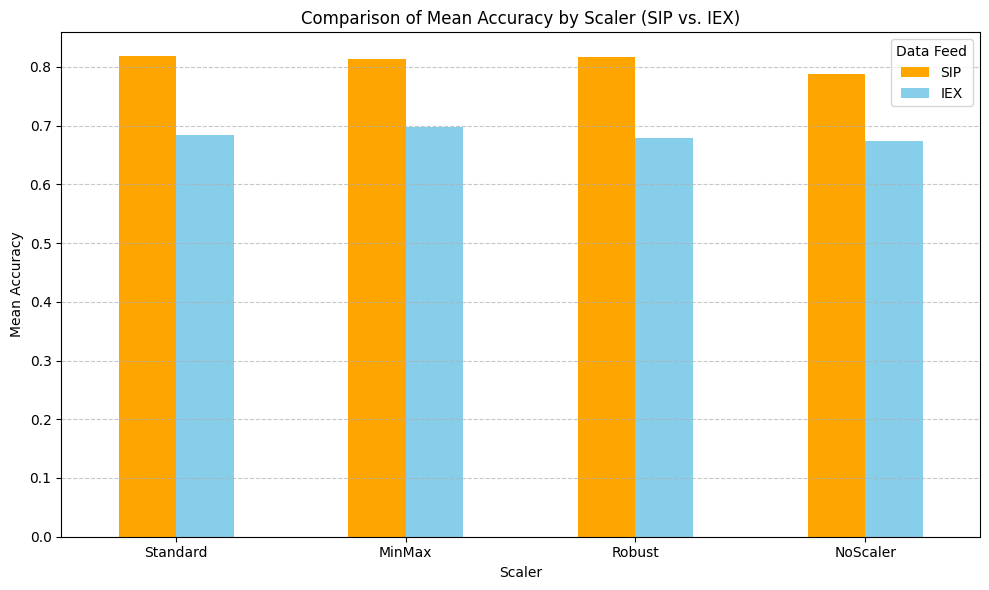
\includegraphics[width=0.95\textwidth]{scaler_comparison.png}
    \caption{Comparison of mean accuracy and loss by scaler between IEX and SIP datasets.}
    \label{fig:scaler_comparison}
\end{figure}

\begin{figure}[H]
    \centering
    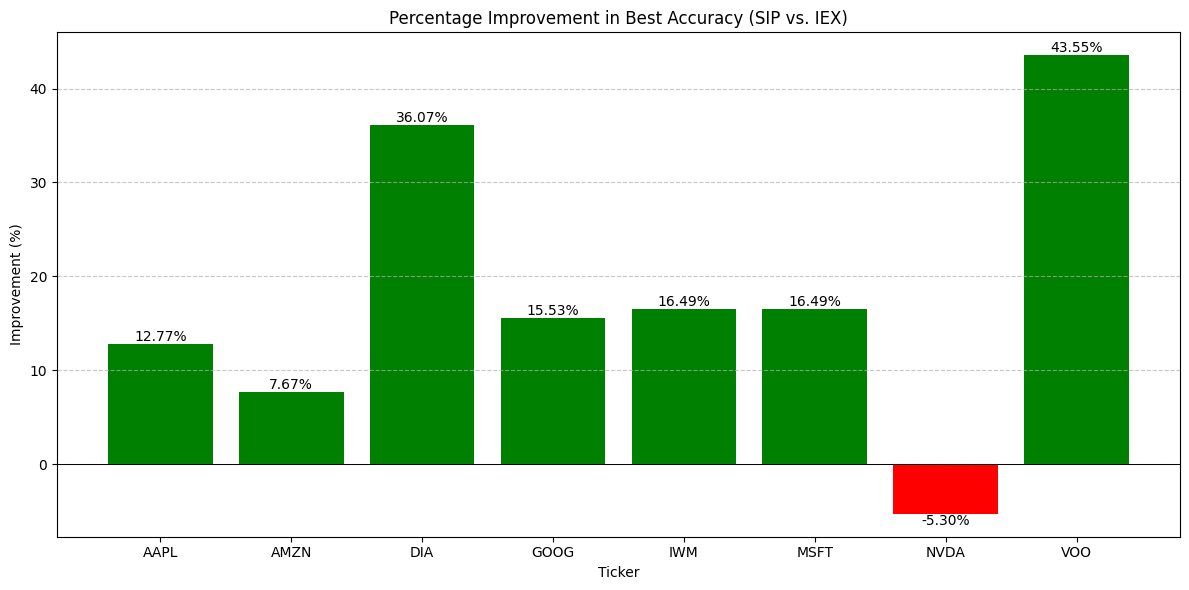
\includegraphics[width=1\textwidth]{accuracy_improvement.png}
    \caption{Percentage improvement in best accuracy per ticker from IEX to SIP. Positive values indicate improved accuracy with SIP data.}
    \label{fig:accuracy_improvement}
\end{figure}

Overall, these visualizations clearly underscore the beneficial role of extended trading hours data in predictive modeling, despite isolated exceptions such as NVDA, which highlight the complexities introduced by high-volatility trading environments.



\subsection{Effectiveness of Scaling Techniques}

Across both the IEX and SIP datasets, data normalization significantly influenced model accuracy and stability, with the optimal scaling technique varying by dataset and asset type. For the IEX dataset, which covers only regular trading hours, the MinMax scaler proved most effective, achieving a mean test accuracy of 0.6981 and a mean test loss of 0.5935. This scaler normalizes features to a fixed range, making it well-suited to the relatively stable and bounded price movements typical of regular trading hours. By reducing the impact of minor fluctuations, the MinMax scaler enhances the model’s ability to detect consistent patterns in this less volatile environment.

In contrast, for the SIP dataset, the Robust scaler outperformed other methods, yielding a mean test accuracy of 0.8201 and a mean test loss of 0.4454. Extended hours often feature lower liquidity, leading to increased volatility, outliers, and price spikes. The Robust scaler, which relies on the median and interquartile range, mitigates the influence of these anomalies, providing a more stable foundation for model predictions. This explains its advantage over alternatives like the MinMax scaler (0.8119 accuracy, 0.4547 loss) and Standard scaler (0.8143 accuracy, 0.4571 loss) in the SIP dataset.

Interestingly, the NoScaler configuration occasionally matched or exceeded scaled approaches, particularly for exchange-traded funds (ETFs) such as DIA (0.8420 accuracy in SIP), IWM (0.8340 in SIP), and VOO (0.8780 in SIP). A similar trend appeared in the IEX dataset, with NoScaler performing best for DIA (0.6200) and IWM (0.7150). This suggests that ETFs, which track broad indices and aggregate multiple stocks, exhibit smoother temporal dynamics that may reduce the need for normalization. Their inherent stability could allow models to effectively leverage raw feature values without additional scaling.

\subsection{Volatility}

To examine the interplay between market volatility and model performance, we computed the annualized volatility for each ticker over the test period (June 7, 2023, to December 30, 2024). In financial contexts, volatility quantifies the dispersion of returns, serving as a proxy for risk. Higher volatility often manifests as larger, more frequent price fluctuations, which can stem from unpredictable events, thereby complicating the identification of consistent patterns for predictive models like LSTMs.

The volatility calculation followed standard financial methodology using daily log returns:


\begin{enumerate}
    \item Compute daily log returns:
    \begin{equation}
    R_t = \ln\left(\frac{P_t}{P_{t-1}}\right),
    \end{equation}
    where \(P_t\) and \(P_{t-1}\) represent closing prices on days \(t\) and \(t-1\), respectively.
    
    \item Calculate daily volatility (\(\sigma_{\text{daily}}\)):
    \begin{equation}
    \sigma_{\text{daily}} = \sqrt{\frac{1}{n-1}\sum_{t=1}^{n}(R_t - \bar{R})^2},
    \end{equation}
    with \(\bar{R}\) as the average daily log return.

    \item Annualize daily volatility assuming 252 trading days per year:
    \begin{equation}
    \sigma_{\text{annualized}} = \sigma_{\text{daily}} \times \sqrt{252}.
    \end{equation}
\end{enumerate}

We then analyzed the correlation between annualized volatility and the best test accuracy, defined as the highest accuracy achieved by the LSTM model for each ticker during the testing phase. As shown in Figure~\ref{fig:volatility_accuracy}, a negative correlation emerged. Highly volatile stocks, such as NVDA, exhibited lower predictive accuracy compared to less volatile tickers like VOO, DIA and MSFT. This suggests that elevated volatility increases the unpredictability of price movements, challenging the LSTM model's ability to identify reliable patterns.

\begin{figure}[H]
    \centering
    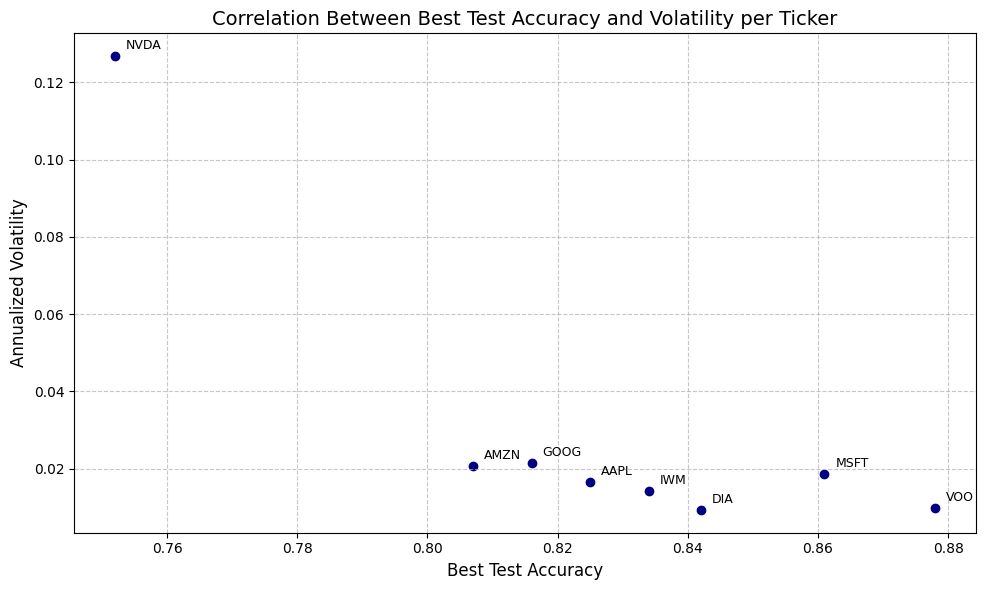
\includegraphics[width=1\textwidth]{volatility_accuracy.png}
    \caption{Correlation between annualized volatility and best test accuracy across tickers. Higher volatility typically corresponds to reduced predictive accuracy.}
    \label{fig:volatility_accuracy}
\end{figure}

The case of NVDA is particularly illustrative. Its predictive accuracy decreased when extended-hours data were included, likely due to increased volatility from events like quarterly earnings announcements and shifting economic conditions. In contrast, ETFs such as VOO and DIA, which benefit from diversification that reduces risk and stabilizes price movements, consistently showed higher accuracy. This highlights volatility as a pivotal factor in forecasting performance.


Overall, this volatility analysis underscores the importance of considering asset-specific volatility characteristics when deploying deep learning models in financial forecasting. Models may require volatility-adaptive architectures or input features explicitly capturing volatility to enhance predictive accuracy in highly turbulent market environments.

\section{Conclusion}

This study comprehensively evaluated the performance of LSTM networks in predicting stock price movements, utilizing multiple scaling methods and incorporating both regular and extended trading hours. The findings revealed clear advantages of including pre-market and post-market trading data (SIP dataset), as evidenced by consistently higher predictive accuracies compared to regular trading hours alone (IEX dataset). These results confirm that extended-hours sessions carry meaningful predictive signals, despite introducing greater market volatility.

The effectiveness of data normalization methods varied significantly by market condition and asset type. MinMax scaling was optimal during regular trading hours due to its suitability for stable and bounded price patterns, whereas Robust scaling outperformed other methods when handling the volatility and outliers characteristic of extended sessions. Notably, exchange-traded funds (ETFs), given their inherently smoother dynamics, often achieved strong performance even without data normalization, underscoring the importance of tailoring preprocessing strategies to asset-specific volatility profiles.

Volatility itself emerged as a pivotal factor influencing predictive accuracy, with higher volatility generally corresponding to lower forecasting reliability. This relationship was especially pronounced in stocks like NVIDIA, which uniquely demonstrated decreased accuracy when models included extended trading data. These observations highlight the complexities of modeling highly volatile assets and suggest the potential benefits of developing volatility-adaptive prediction models or explicitly incorporating volatility measures as inputs. 

In conclusion, effective stock market prediction using LSTM networks requires careful consideration of trading session selection, asset-specific volatility, and normalization techniques. Future research building upon these findings promises further advances in accuracy, adaptability, and practical utility in financial forecasting.

\newpage

\includepdf[pages=-]{Attachments.pdf}
\newpage

%
% ---- Bibliography ----
%
% BibTeX users should specify bibliography style 'splncs04'.
% References will then be sorted and formatted in the correct style.

\bibliographystyle{splncs04}
\bibliography{referencias}

\end{document}
